\documentclass[12pt]{article}

\usepackage[a4paper, total={6.5in,10in}]{geometry}
\usepackage{xcolor}
\usepackage{graphicx}
\usepackage{blindtext}
\usepackage{amsmath}
\usepackage{amsfonts}
\usepackage{caption}
\usepackage{subcaption}
\usepackage{listings}
\usepackage{subfig}

\pagecolor[rgb]{0.2,0.2,0.2}
\color[rgb]{0.95,0.95,0.95}

\begin{document}


\begin{center}
\begin{huge}
\textbf{Master's Encyclopedia}
\end{huge}
\\~\\
\noindent\rule{16.5cm}{0.4pt}
\end{center}

\begin{flushleft}

\section{Introduction}
\qquad The purpose of this document is to provide detailed explanations the most important points of the paper's provided by Dr. Protas for my masters thesis research. Each section is intended to provide the relevant definitions, derivations, and theory of the topic as it relates to my research. This document is not intended as a comprehensive review of each subject. Segments of this document are taken directly from textbooks, papers, and online sources and so is not my original work.

\section{3D Torus}
\qquad The 3D torus is denoted by the symbol, $\Omega = \mathbb{T}^3 := (\mathbb{R}/\mathbb{Z})^3$. The domain of the torus is usually $\boldsymbol x\in [0,1]^3$ or $\boldsymbol x\in [0,2\pi]^3$ where $\boldsymbol x$ is a vector. The 3D torus has periodic boundaries. The functions defined on $\Omega$ are usually periodic, but do not necessarily need to be.
\\~\\
\qquad Because of the periodic boundary, each pair of opposite faces on $\Omega$ are actually the same face. Therefore, the value of a periodic function is the same on opposite faces. However, the normal vector in the surface integral is, by convention, outward-pointing. Therefore, the surface integral over one face will be exactly cancelled by the integral over the opposite face. This means the surface integral of a periodic function on $\Omega$ is zero.
\\~\\
\qquad The resolution of a simulation describes the number of points in the grid. It is denoted by the symbol $N^3$ where $N$ is the number of points along each axis. Typically the simulations will use a resolution of $128^3$, $256^3$, $512^3$, or $1024^3$. The simulations for my Masters thesis will use uniform grids. However, some simulations utilize adaptive grids which increase the local resolution near points of interest.

\section{Smooth and Analytic Functions}

\qquad The smoothness of a function is a property measured by the number of continuous derivatives it has over its domain. The smoothness of a function is denoted by the symbol, $C^k$ where the function has a k-th order continuous derivative. The function of class $C^\infty$ is an infinitely differentiable function. 
\\~\\
\qquad An analytic function is a function that is differentiable at every point in a region, and it can be represented by a convergent power series. There are both real and complex analytic functions. Both types are infinitely differentiable and so are in $C^\infty$. However, not all $C^\infty$ functions are analytic. For example,
\[ f(x) = \begin{cases} 
      e^{-1/x} & \text{if }x>0, \\
      0 & \text{if }x\leq 0. \\ 
   \end{cases}
\]
This function is smooth as it has continuous derivatives of all orders at every real number $x$. However, the function is not analytic.

\section{Fourier Analysis}
\subsection{Fourier Transform}

\qquad The Fourier Transform (FT) is a mathematical tool that decomposes a function into its constituent frequencies. This transforms the function from physical space to its frequency domain or Fourier Space. The Fourier transform of a function $u(x)$, $x\in \mathbb{R}$ is the function $\hat{u}(k)$ defined by,
$$\hat{u}(k) = \int_{-\infty}^{\infty}e^{-ikx}u(x)dx, \qquad k\in \mathbb{R}.$$
The number $\hat{u}(k)$ can be interpreted as the amplitude density of $u$ at wavenumber $k$. Below is a visualization of the Fourier transform of a function. 
\\~\\
\begin{figure}[h!]
\centering
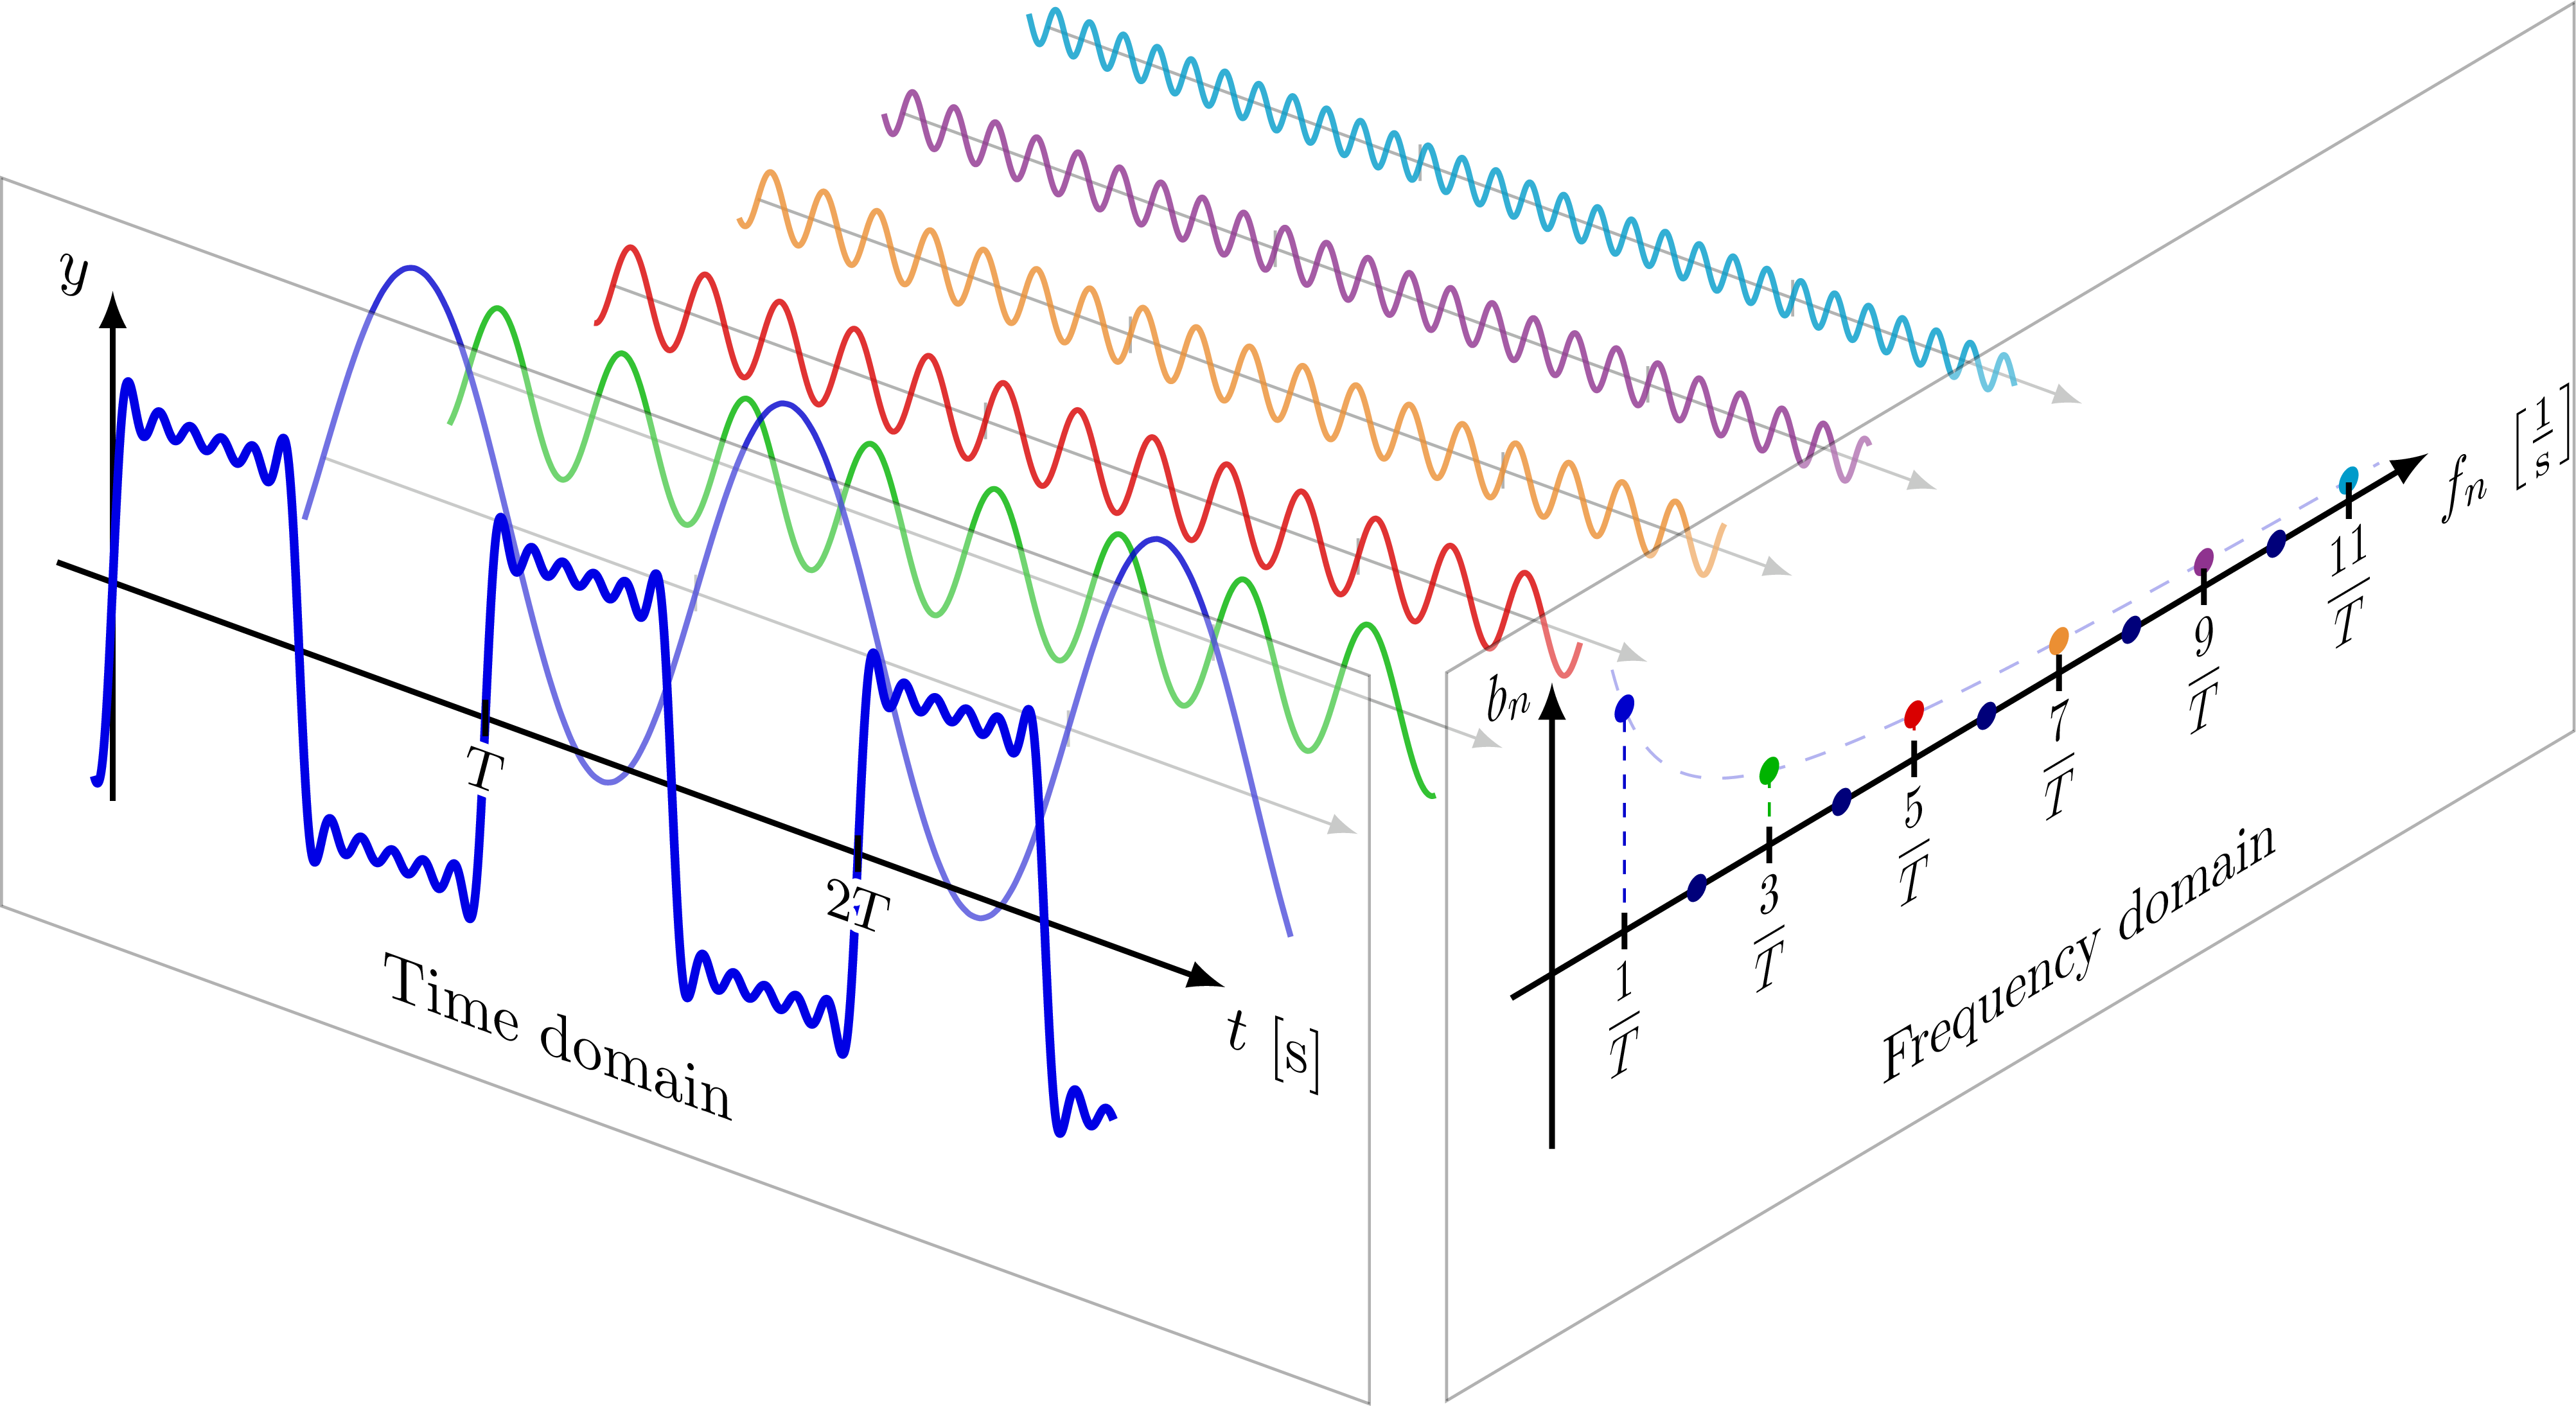
\includegraphics[scale=0.08]{fourier_series_visualization.png}
\end{figure}

\subsection{Inverse Fourier Transform}
Conversely, we can reconstruct $u$ from $\hat{u}$ by the inverse Fourier transform,
$$u(x) = \frac{1}{2\pi}\int_{-\infty}^{\infty}e^{ikx}\hat{u}(k)dk, \qquad x\in\mathbb{R}.$$
The Fourier transform and inverse Fourier transform are defined over continuous unbounded space ($x$) and continuous unbounded wavenumbers ($k$). 
\\~\\
The $L^2$-norms of $u$ and $\hat{u}$ are related by Parseval's equality,
$$\|\hat{u}\| = \sqrt{2\pi}\|u\|$$

\subsection{Semi-discrete Fourier Transform}
\qquad In numerical simulations we utilize discrete space, not continuous space. Therefore, we must consider $x \in h\mathbb{Z}$ rather than $x\in R$. Precise analogues of the Fourier transform and its inverse exist for this case. However, because the spatial domain is discrete, the wave number k will no longer range over all of $\mathbb{R}$. Rather, the wavenumber domain is a bounded interval of length $2\pi/h$. One suitable case for this the range $x\in [-\pi/h,\pi/h]$. For a function $v$ defined on $h\mathbb{Z}$ with value $v_j$ at $x_j$, the semi-discrete Fourier transform is defined by,
$$\hat{v}(k) = h\sum_{-\infty}^{\infty}e^{-ikx_j}v_j, \qquad k\in [-\pi/h,\pi/h].$$

\subsection{Inverse Semi-discrete Fourier Transform}
The inverse semi-discrete Fourier transform is,
$$v_j = \frac{1}{2\pi}\int_{-\pi/h}^{\pi/h}e^{ikx_j}\hat{v}(k)dk, \qquad j\in\mathbb{Z}.$$

\subsection{Discrete Fourier Transform}

\qquad Numerical simulations not only utilize discrete space, but finite discrete space. Therefore we must consider $x\in h\mathbb{Z}$ for a finite number of terms. For this case we use the Discrete Fourier Transform,
$$\hat{v}(k) = \sum_{j=0}^{N-1}v_j e^{-2\pi i k j/N}, \qquad j\in\mathbb{Z}$$

\subsection{Inverse Discrete Fourier Transform}

The inverse discrete Fourier transform is,
$$v_j = \frac{1}{N}\sum_{k=0}^{N-1} \hat{v}(k)e^{2\pi ik j/N}, \qquad j\in\mathbb{Z}$$

\subsection{Fourier Series}

\subsection{Fourier Expansion}

\qquad We must also consider the case of a function defined on a periodic domain $x\in\Omega$. A function in this domain can be expressed with the Fourier expansion,
$$u(x) = \sum_{k\in \mathbb{Z}^3}\hat{u}_k e^{ikx}$$
where the coefficients $\hat{u}_k$ are complex numbers satisfying the condition
$$\hat{u}_k = \overline{\hat{u}_{-k}} \qquad \text{for all}  \qquad k \in \mathbb{Z}^3$$
imposed to ensure that $u$ is real. If needed, the Fourier coefficients $\hat{u}_k$ can be computed explicitly via the integral,
$$\hat{u}_k = \frac{1}{(2\pi)^3}\int_{\Omega}e^{-ikx}u(x)dx.$$
The Fourier coefficients represent the amplitude and phase at each frequency of the series. From the Payley-Wiener theorem, if $u(x)$ is real analytic, then its Fourier coefficients decay exponentially and conversely, if a Fourier expansion has exponentially decreasing coefficients then it is real analytic.

\subsection{Fast Fourier Transform}

The Fast Fourier Transform is an algorithm for computing the discrete Fourier transform. The most common FFT algorithm is the Cooley-Tukey algorithm.

\subsection{Inverse Fast Fourier Transform}

The Inverse Fast Fourier Transform is an algorithm for computing the inverse discrete Fourier transform.

\subsection{Fourier Filter}

The Fourier filter is a type of filtering function that is based on manipulation of specific frequency components of a signal. It works by taking the Fourier transform of the signal, then attenuating or amplifying specific frequencies, and finally inverse transforming the result.

\subsection{Fourier Mode}

The Fourier Mode is ...

\subsection{Randomization in Fourier Space}

\section{Initial Conditions}

There are a variety of initial conditions that can be used in our research. The initial condition is denoted by the symbol, $\eta$. There are several key properties common to these initial conditions. 
\\~\\
The first is that each initial condition is periodic on $\Omega$. We also assume, without loss of generality, that
$$\int_{\Omega}\eta dx = 0$$
WHAT IS IMPORTANT ABOUT THIS. This property remains true for all time $t$. The initial conditions must be divergence free, 
$$\nabla \cdot \eta = 0$$

\subsection{Taylor-Green Vortex}

\qquad The Taylor–Green vortex has been widely used as a candidate for potential blow up in Euler flows, however,it is still an open question whether this initial condition can indeed lead to a singularity formation in a finite time. The formula for the Taylor-Green vortex is,
$$\eta := \begin{bmatrix}
\sin(2\pi)\cos(2\pi y)\cos(2\pi z)\\
-\cos(2\pi x)\sin(2\pi y)\cos(2\pi z)\\
0
\end{bmatrix}$$
Below is a visualization of the z-component vorticity of the Taylor-Green Vortex.

\begin{figure}[h!]
\centering
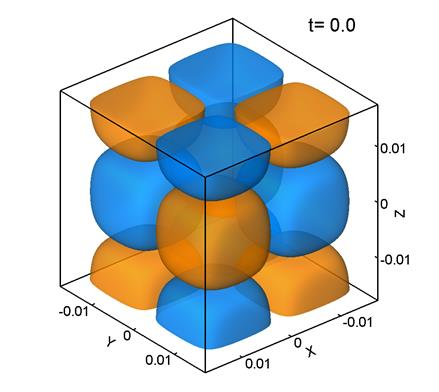
\includegraphics[scale=0.75]{Taylor_Green_Vortex.jpg}
\end{figure}


\subsection{Kerr}

The Kerr initial condition represents two perturbed anti-parallel vortex tubes located symmetrically with respect to the xy-plane such that $\omega(x,y,z)=-\omega(x,y,-z)$. It is given by the formula,
$$\eta := \nabla \times (|D|^{-2}\omega$$
where
$$\omega = 8G\omega(r)[\omega_1,\omega_2,\omega_3]^T$$
where G is the Fourier filter defined by 
$$\hat{G}_j = \exp(-0.05(j_1^4 + j_2^4 + j_3^4))$$
and
\[ \omega(r) = \begin{cases} 
      \exp[(-r^2/(1-r^2))+r^4(1+r^2+r^4)] & r<1, \\
      0 & r\geq 1. \\ 
   \end{cases}
\]
where
$$r = \frac{1}{R}\sqrt{[x-x(s)]^2 + [z-z(s)]^2}$$
$$x(s) = \delta_x\cos(\pi s/L_x)$$
$$z(s) = z_0$$
$$s(y) = y_2 + L_y\delta_{y1}\sin(\pi y_2/L_y)$$
$$y_2(y) = 4\pi y+L_y\delta_{y2}\sin(4\pi y)/L_y)$$
$$\omega_1 = \frac{-\pi\delta_x}{L_x}[1+\pi\delta_{y2}\cos(\pi(4\pi y)/L_y)]]*[1+\pi\delta_{y1}\cos(\pi y_2/L_y)]\sin(\pi s/L_x)$$
$$\omega_2 = 1$$
$$\omega_3 = 0$$
We choose the parameters,
$$\delta_{y1} = 0.5, \delta_{y2}=0.4, \delta_x=-1.6, z_0=1.57$$
$$R=0.75, L_x = L_y = 4\pi, L_z = 2\pi$$
A visualization of the vorticity of the Kerr initial condition is shown below. The tube is the isosurface at 60\% of the maximum vorticity. 
\begin{figure}[h!]
\centering
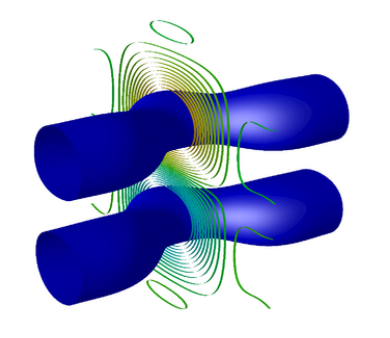
\includegraphics[scale=1.0]{Kerr_Vortex.png}
\end{figure}
\subsection{Hou}

The Hou axisymmetric initial condition is given by the equation,
$$\eta := Gu_\theta e_\theta$$
where $e_\theta$ is the unit vector in the azimuthal direction of the cylindrical coordinate system and $u_\theta$ is the angular velocity component given by,
\[ u_\theta = \begin{cases} 
      r\exp(-r^2/(1-r^2))\frac{12000(1-r^2)^{18}\sin(2\pi z)}{1+12.5\sin^2(\pi z)}& r<1, \\
      0 & r\geq 1. \\ 
   \end{cases}
\]
where 
$$r = \frac{\sqrt{x^2+y^2}}{0.9}$$
A visualization of the Hou initial condition is shown below. FIND VISUALIZATION.

\subsection{Random}

The random initial condition is defined by the equation,
$$\eta := P_L v_{\text{rand}} := v_{\text{rand}} - \nabla \Delta^{-1}(\nabla \cdot v_{\text{rand}})$$
where $P_L$ is the Leray projector with the property that for any $\omega\in H^1(\mathbb{T}^3)$, $\nabla\cdot (P_L \omega) = 0$, and $v_{\text{rand}}$ is given by,
$$v_{\text{rand}} = \begin{bmatrix}
v_1\\
v_2\\
v_3
\end{bmatrix} = 
\begin{bmatrix}
\sum_{|j_1|+|j_2|+|j_3|\leq N_0}e^{-|j|/(4\pi)}e^{i2\pi\theta_1(j_1)}e^{i2\pi j\cdot x}+c.c.\\
\sum_{|j_1|+|j_2|+|j_3|\leq N_0}e^{-|j|/(4\pi)}e^{i2\pi\theta_2(j_2)}e^{i2\pi j\cdot x}+c.c.\\
\sum_{|j_1|+|j_2|+|j_3|\leq N_0}e^{-|j|/(4\pi)}e^{i2\pi\theta_3(j_3)}e^{i2\pi j\cdot x}+c.c.
\end{bmatrix}$$
where $\theta_1$, $\theta_2$, and $\theta_3$ are $N_0$-dimensional random variables with uniform distributions on $[0,1]^{N_0}$. In practice, we use $N_0=64$.

\section{Supremum and Infimum}

\qquad The supremum, denoted as $\text{sup} f(x)$, represents the smallest upper bound of the values attained by the function over a given domain. It is the largest value that the function can achieve. The infimum, denoted as $\text{inf} f(x)$, represents the greatest lower bound of a set, meaning the largest number that is less than or equal to all elements in the set.
\\~\\
\qquad The essential supremum, $ess sup f(x)$, is the smallest value that is greater than or equal to the function values everywhere while ignoring what the function does at a set of points of measure zero. The essential infimum, $ess inf f(x)$, is the largest value that is greater than or equal to the function values everywhere while ignoring what the function does at a set of points of measure zero.
\\~\\
\qquad The limit superior, denoted $\limsup f(x)$, is the supremum of a functions limit. Therefore it is the smallest upper bound of the values attained by the function over a given domain as it approaches the limit argument. The limit infimum, denoted $\liminf f(x)$,  is the infimum of a functions limit. Therefore it is the largest lower bound of the values attained by the function over a given domain as it approaches the limit argument.

\section{Functional Analysis}

\subsection{Metric Spaces}

A metric space is a set X with a metric d,
$$d:X\times X \rightarrow [0,\infty)$$
with the conditions that, given $x,y,z\in X$,
$$d(x,y)=0 \Leftrightarrow x=y$$
$$d(x,y) = d(y,x)$$
$$d(x,y) \leq d(x,z)+d(z,y)$$
An open ball around x is the set,
$$B_\epsilon(x) := \{y\in X |  d(x,y)<\epsilon\}$$
where $\epsilon > 0$. A set $A\subset X$ is called open if for each $x\in A$ there is an open ball with $B_\epsilon(x)\subset A$. A boundary point is a point $x\in X$ is a boundary point for A if for all $\epsilon>0$, $$B_\epsilon(x)\cap A \neq \emptyset$$ 
and 
$$B_\epsilon(x)\cap A^c \neq \emptyset$$
The boundary of $A$ is the set that contains all boundary points for A and is denoted as $\partial A$. A set $A$ is closed if $A^c$ is open. The closure of a is $\overline{A} = A \cup \partial A$. Let $D$ be a bounded open subset of $\mathbb{R}^n$, and $\overline{D}$ be a bounded closed subset of $\mathbb{R}^n$. 

\subsection{Complete Space}

\qquad A sequence $x_1,x_2,x_3,...\in X$, where $X$ is a metric space, is called Cauchy if for every positive real number r there is a positive integer $N$ such that for all positive integers $m,n>N$, $d(x_m,x_n)<r$. A metric space is complete if every Cauchy sequence in X has a limit that is also in X.

\subsection{Norms}

A map $\|\cdot\|: X\rightarrow [0,\infty)$ is called a norm if,
$$\|x\| = 0 \Leftrightarrow x=0$$
$$\|\lambda x\| = \lambda| \|x\|$$
$$\|x+y\| \leq \|x\| + \|y\|$$
A vector space with a norm is called a normed space. If $\|\cdot \|$ is the norm of the vector space X, then 
$$d_{\|\cdot\|}(x,y) := \|x-y\|$$
defines a metric for the set X. Therefore, a normed space is a type of metric space.

\subsection{Function Spaces}

A function space is a set of functions between two fixed sets.

\subsection{Banach Spaces}

A Banach space is a complete normed metric space. The space $C^0(D)$ is the space of continuous functions on D. The space $C^0(\overline{D})$ of continuous functions on $\overline{D}$ with norm,
$$||u||_{C^0(\overline{D})}:=\sup_{x\in \overline{D}}|u(x)|$$
is a Banach space. The space of $k$-times continuously differential functions on $\overline{D}$ is a Banach space when equipped with the norm,
$$||u||_{C^k(\overline{D})}:=\sum_{|\alpha|\leq k}||\partial^\alpha u||_{C^k(\overline{D})}$$
When X is a Banach space we denote the space of all continuous functions from [0,T] into X by $C([0,t];X)$, equipped with the norm,
$$\|u\|_{C([0,t];X)} := \sup_{t\in[0,T]}\|u(t)\|_X$$

\subsection{Lebesgue Spaces}

\qquad Lebesgue spaces are function spaces defined using a natural generalization of the p-norm for finite-dimensional vector spaces. They are a type of Banach Space. By $L^p(D)$, where $1\leq p < \infty$, we denote the standard Lebesgue space of measurable p-integrable functions with the norm, 
$$\|u\|_{L^p} := \left( \int_D |u(x)|^p dx \right)^{1/p}$$
The space $L^\infty(D)$ of essentially bounded functions on $D$ is equipped with the standard norm
$$\|u\|_{L^\infty} := \text{ess sup}|u|$$

\subsection{Sobolev Spaces}

\qquad A Sobolev space is a vector space of functions equipped with a norm that is a combination of $L^p$-norms of the function together with its derivatives up to a given order. Let $1\leq p <\infty$. The space $W^{1,p}(D)$ consists of all those functions $u\in L^p(D)$ all of whose first weak derivatives $\partial_i u$ exist and are in $L^p(D)$. The norm in $W^{1,p}(D)$ is given by,
$$\|u\|_{W^{1,p}} := \left( \int_D |u(x)|^p + \sum_{i=1}^n \int_D |\partial_i u(x)|^p dx \right)^{1/p}$$
The space $W^{k,p}(D)$ is the space of functions $u\in W^{k-1,p}(D)$ all of whose first weak derivatives also belong to $W^{k-1,p}(D)$. The standard norm in $W^{k,p}(D)$ is given by
$$\|u\|_{W^{k,p}}^p := \sum_{|\alpha|\leq k}\|\partial \alpha u\|_{L^p}^p.$$
On $\Omega$ we can make use of the Fourier expansion of $u$. The $L^2$-norm is,
$$\|u\|^2 = (2\pi)^3\sum_k|\hat{u}_k|^2$$
We will often use the $L^2$-based Sobolev spaces $W^{k,2}$. We adopt the notation,
$$H^k(D) := W^{k,2}(D)$$
$$H_0^k(D) := W_0^{k,2}(D)$$
We can use the gradient of $u$ to obtain,
$$\|\nabla u\|^2 = (2\pi)^3\sum_{k\in \mathbb{Z}^3}|k|^2|\hat{u}_k|^2$$
For $s\geq 0$ the Sobolev space $H^s(\Omega)$ consists of all the functions for which the norm,
$$\|u\|_{H^s}^2 := (2\pi)^3\sum_{k\in\mathbb{Z}^3}(1+|k|^{2s})|\hat{u}_k|^2$$
is finite. For any $u\in H^s(\Omega)$,
$$\|u\|_{\dot{H}^s}^2 := (2\pi)^3 \sum_{k\in\mathbb{Z}^3}|k|^{2s}|\hat{u}_k|^2$$

\subsection{Hilbert Spaces}

\qquad A Hilbert space is a vector space equipped with an inner product operation. A Hilbert space is a type of Banach space where the norm is derived from an inner product. The spaces $H^k(D)$ and $H_0^k(D)$ are Hilbert spaces with the inner product,
$$<u,v>_{H^k} := \sum_{0\leq |\alpha|\leq k}<\partial^\alpha u, \partial^\alpha v$$,
and the corresponding norm,
$$\|u\|_{H^k}^2 = <u,u>_{H^k} = \sum_{0\leq |\alpha|\leq k}\|\partial^\alpha u\|^2.$$

The space Lebesgue space $L^2(D)$ is a Hilbert space when equipped with the inner product,
$$<u,v> := \int_D u(x)\cdot v(x) dx$$

\subsection{Gevrey Subspace} 
\subsection{Manifolds}

\section{Strong vs Weak Solutions}

\section{Time Stepping}
\subsection{Runge-Kutta-4}
 
\section{The Adjoint Method} 
\subsection{The Gateaux Directional Differential}
 
\section{Navier-Stokes Equations}

\section{Navier-Stokes-Voigt Equations} 
 
\section{Euler's Equations}
same difficulties as the 3D Navier-Stokes equations in the case of large Reynolds numbers.

\section{Euler-Voigt Equations}
\subsection{$\alpha$-Energy}
\subsection{Linearization}

\section{Burgers Equation}
\subsection{Viscid}
\subsection{Inviscid}

\section{Blow-up Criteria}
\subsection{Beale-Kato-Majda Criterion}
\subsection{Vorticity Criterion}
\subsection{Voigt-type Criterion}
\subsection{Enstrophy}


\section{Optimization Problems}
\section{Brent's Minimization Method}

\qquad Given a function $f$ that depends on one or more independent variables find the value of those variables where $f$ takes on a minimum value. Use this variables calculate the minimum value of $f$. In general, finding a global minimum of a function is very difficult. It is made more difficult by the fact that we do not have the derivative of the function. To solve this problem we use Brent's method. 
\\~\\
Before describing Brent's Method, we must first bracket a minimum. A minimum is known to be bracketed only when there is a triplet of points, $a<b<c$ or $c<b<a$, such that $f(b)$ is less than both $f(a)$ and $f(c)$. In this case, we know that the function has a minimum in the interval $(a,c)$. The initial bracketing of a minimum is done by METHOD WE USED.
\\~\\
\qquad We must also describe the Golden Search method as it is a tool used by Brent's Method. The general procedure is to choose a new point x, either between $a$ and $b$ or between $b$ and $c$. Suppose we make the latter choice. Then we evaluate $f(x)$. If $f(b)<f(x)$, then the new bracketing triplet is $(a,b,x)$. If $f(b)>f(x)$, then the new triplet is $(b,x,c)$. In all cases, the middle point of the new triplet is the abscissa whose ordinate is the best minimum achieved so far. We continue the process until the distance between the two outer points of the triplet is below some chosen tolerance. The question remains, how do we choose the new point x, given $(a,b,c)$. The answer is to choose a point which is a fraction $0.38197$ into the larger of the two intervals, from the central point of the triplet. The derivation can be found in Section 10.2 of Numerical Recipes.
\\~\\
\qquad We can now describe Brent's Method. If the function is nicely parabolic near the minimum then a parabola fitted through any three points ought to take us in a single leap to the minimum, or at least very near to it. Since we want to find an abscissa rather than an ordinate, the procedure is called inverse parabolic interpolation. The formula for the abscissa $x$ that is the minimum of a parabola through three points $f(a)$, $f(b)$, and $f(c)$ is
$$x = b - \frac{1}{2}\frac{(b-a)^2[f(b)-f(c)]-(b-c)^2[f(b)-f(a)]}{(b-a)[f(b)-f(c)]-(b-c)[f(b)-f(a)]}$$
\qquad This formula fails only if the three points are collinear. Brent's Method works by using Golden Search when the function is not cooperative, but uses the formula above when the function allows. Brent's Method uses six variables, $a$, $b$, $u$, $v$, $w$, and $x$. The minimum is bracketed between $a$ and $b$. $x$ is the point with the very least function value found so far, or the most recent one in case of a tie. $w$ is the point with the second least function value. $v$ is the previous value of $w$. $u$ is the point at which the function was evaluated most recently. There is an addition point $x_m$ which is the midpoint between $a$ and $b$, but the function is not evaluated here. 
\\~\\
\qquad The Brent's Method code can be found in Section 10.3 of Numerical Recipes. Here is an overview of the algorithm. 
\\~\\
1) Initialize the maximum number of allowed iterations. Initialize, $a$, $b$, $x$, $w$, $v$, and the values of $f$ at $w$, $v$, and $x$ to $f(x)$.
\\~\\
2) Begin the iteration. Calculated $x_m$. Test if the interval is less than the tolerance. If it is return the value of $x$ and terminate.
\\~\\
3) Construct a parabolic fit. Check the acceptability of the fit to determine if it should use the Golden Search Method. Use this to find the step size for finding the next value to check. Use this value to update the variables. Repeat from step 2 until max iterations is reached or it terminates for the interval test.

\section{Linear Conjugate Gradient}

The conjugate gradient method is an iterative method for solving a linear system of equations
$$Ax = b$$
where A is an $n\times n$ symmetric positive definite matrix. The problem can be stated equivalently as the following minimization problem:
$$\min \phi(x):=\frac{1}{2}x^TAx -b^Tx$$
\qquad This equivalence will allow us to interpret the conjugate gradient method either as an algorithm for solving linear systems or as a technique for minimizing convex quadratic functions, which is what we will be doing for the research project. For this problem, the gradient of $\phi$ equals the residual of the linear system,
$$\nabla\phi(x) = Ax-b := r(x)$$
A set of nonzero vectors is said to be conjugate with respect the symmetric positive definite matrix A if,
$$p_i^TAp_j = 0, \qquad \text{for all} i\neq j.$$
\qquad The importance of this set lies in the fact that we can minimize $\phi$ in at most n steps by successively minimizing it along the individual directions in a conjugate set. The conjugate gradient method has a very special property, namely that it can compute a new vector $p_k$ by using on the previous vector $p_{k-1}$. It does not need to know all the previous elements of $p$. This property allows it minimize storage and computational cost. The search direction at iteration k is given by,
$$p_k = -r_k + \beta_kp_{k-1}$$
where $\beta_k$ is a scalar "momentum" term that enforces the conjugacy of consecutive search directions. The step size is computed explicitly using a formula. We use the non-linear conjugate gradient method so further detail is not needed.

\section{Non-Linear Conjugate Gradient}

\qquad The Conjugate Gradient method is a minimization algorithm for the convex quadratic function $\phi$. The question becomes, how do we adapt the approach to minimize general convex functions, or even general non-linear functions f. This is done with the Fletcher-Reeves and Polak-Ribiere Methods. The Fletcher-Reeves method makes two changes to extend the algorithm to non-linear functions. First the step length is calculated using a line search that identifies an approximate minimum of the non linear function $f$ along $p_k$. This is the method we use for our research. We use Brent's method to find the value of the step size. Second we replace the residual r with the gradient of the non-linear objective $f$.
\\~\\
The Polak-Ribiere Method varies in the way it calculates $\beta_k$. The formula we use is in the section below.

\section{Riemannian Conjugate Gradient Method}

\qquad The Riemannian Conjugate Gradient Method is taken from the paper, Systematic Search for Singularities in 3D Euler Flows. 

\section{Spectral Methods}

\pagebreak

\section{Paper Summary}
\begin{center}
\begin{large}
\textbf{A computational investigation of the finite-time blow-up of the 3D incompressible Euler equations based on the Voigt regularization}
\\~\\
\end{large}
\textbf{Adam Larios, Mark R. Petersen, Edress S. Titi, Beth Wingate}
\\~\\
\end{center}

\qquad This paper examines two blow-up criteria for the 3D incompressible Euler-Voigt equations with periodic boundary conditions $\Omega := [0,1]^3$. It also investigates the analogous criteria for blow-up of the 1D Burgers equation, where blow-up is well known to occur. The result of the present work is that extrapolation to $\alpha$ suggests the development of a singularity in the 3D Euler equations corresponding to $T^* \approx 4.4 \pm 0.2$.
\\~\\
If the blow-up criteria are met, then the 3D Euler equations must develop a singularity at or before time $T^*$. The blow-up criteria are,
$$\sup_{t\in[0,T^*]}\limsup_{\alpha\rightarrow 0^+}(\alpha\|\nabla\textbf{u}^\alpha(t)\|_{L^2}) > 0$$
and
$$\limsup_{\alpha\rightarrow 0^+} \left( \alpha \sup_{t\in [0,T^*]}\|\nabla\textbf{u}^\alpha(t)\|_{L^2} \right) > 0$$
The second condition is a stronger criterion and so singularities indicated by the first will also be indicated by it.
\\~\\
\qquad All simulations were carried out using a pseudospectral method on the periodic unit cube, namely with derivatives computed in Fourier space, and products computed in physical space with the 2/3’s dealiasing rule applied. Time stepping for the inviscid equations was done using a fully explicit fourth-order Runge–Kutta-4 scheme complying with the advective CFL condition. The Euler-Voigt simulations used Taylor-Green initial conditions with resolutions of $1024^3$ and $512^3$.
\\~\\
The paper also shows that the 1D Burgers equation developes a singularity at time $T^*=1$ for initial condition $u_0(x) = -\sin(x)$.

\section{Paper Summary}
\begin{center}
\begin{large}
\textbf{Maximum amplification of enstrophy in three-dimensional Navier-Stokes flows}
\\~\\
\end{large}
\textbf{Di Kang, Dongfang Yun, Bartosz Protas}
\\~\\
\end{center}
\qquad This paper uses a systematic search for potential singularities in 3D Navier-Stokes flows. It uses Enstrophy as its criteria for identifying blow-up.

\section{References}

\end{flushleft}
\end{document}